\chapter{Grupos resolubles} % Solución para ecuaciones con radicales
\begin{definicion}[Serie de un grupo]
    Sea $G$ un grupo, una serie de $G$ es una cadena de subgrupos $G_0,G_1,\ldots, G_r$ de forma que:
    \begin{equation*}
        G = G_0 > G_1 > G_2 > \ldots > G_r = \{1\}
    \end{equation*}
    Y diremos que la serie tiene longitud $r$.
\end{definicion}

\begin{ejemplo}
    En $S_3$, podemos considerar la serie:
    \begin{equation*}
        S_3 > A_3 > \{1\}
    \end{equation*}

    Donde:
    \begin{equation*}
        A_3 = \langle (1\ 2\ 3) \rangle  = \{1, (1\ 2\ 3), (1\ 3\ 2)\}
    \end{equation*}
\end{ejemplo}

\begin{definicion}[Refinamiento]
    Sea $G$ un grupo, consideramos sobre él dos series:
    \begin{equation}\label{eq:serie_1}
        G = G_0 > G_1 > G_2 > \ldots > G_r = \{1\}
    \end{equation}
    \begin{equation}\label{eq:serie_2}
        G = H_0 > H_1 > \ldots > H_s = \{1\}
    \end{equation}
    Diremos que~(\ref{eq:serie_1}) es un refinamiento de~(\ref{eq:serie_2}) si todo grupo que aparece en~(\ref{eq:serie_2}) también aparece en~(\ref{eq:serie_1}). Ha de ser por tanto $r\geq s$.\\

    \noindent
    Decimos que una serie es un refinamiento propio de la primera si en la primera serie hay grupos que no aparecen en la segunda.
\end{definicion}

\begin{ejemplo}
    En $A_4$, podemos considerar:
    \begin{equation*}
        A_4 > V > \{1\}
    \end{equation*}
    Que podemos refinarla con:
    \begin{equation*}
        A_4 > V > \langle (1\ 2)(3\ 4) \rangle > \{1\}
    \end{equation*}
    Que es un refinamiento propio de la primera serie.
\end{ejemplo}

\begin{definicion}[Serie propia]
    Sea $G$ un grupo y consideramos una serie de $G$, se dice que la serie es propia si todas las inclusiones entre los subgrupos de $G$ que consideramos son propias.\\

    \noindent
    Además, la serie se dice normal si todas las relaciones de subgrupo que aparecen son de subgrupo normal, es decir, si $G_{i-1}\lhd G_i$ para todo $i \in \{1,\ldots,r\}$.
\end{definicion}

\begin{ejemplo}
    Ejemplos de series normales son:
    \begin{gather*}
        S_3 \rhd A_3 \rhd \{1\} \\
        A_4 \rhd V \rhd \{1\} \\
        A_4 \rhd V \rhd \langle (1\ 2)(3\ 4) \rangle \rhd \{1\}
    \end{gather*}
\end{ejemplo}

\begin{definicion}[Factores de una serie]
    En una serie normal podemos considerar cocientes, a los que llamaremos factores de la serie:
    Si $G = G_0 \rhd G_1 \rhd \ldots \rhd G_r$ es una serie, los factores de la serie serán los cocientes:
    \begin{equation*}
        G_{i-1}/G_i \qquad \forall i \in \{1,\ldots,r\}
    \end{equation*}
    LLamaremos también índices de la serie a los índices de los factores, que lo notaremos como:
    \begin{equation*}
        \stackrel{i}{\rhd}
    \end{equation*}
\end{definicion}

\begin{ejemplo}
    Por ejemplo, en la serie:
    \begin{equation*}
        S_3 \rhd A_3 \rhd \{1\}
    \end{equation*}
    Tenemos los factores:
    \begin{gather*}
        S_3/A_3 \cong C_2 \\
        A_3/\{1\} \cong A_3
    \end{gather*}
\end{ejemplo}

\begin{definicion}
    Sea $G$ un grupo, dos series normales de $G$:
    \begin{gather*}
        G = G_0 \rhd G_1 \rhd \ldots \rhd G_r = \{1\} \\
        G = H_0 \rhd H_1 \rhd \ldots \rhd H_r = \{1\}
    \end{gather*}
    Se dice que son isomorfas si $r=s$ y existe $\sigma\in S_r$ de forma que:
    \begin{equation*}
        G_{i-1}/G_i \cong H_{\sigma(i)-1}/H_{\sigma(i)} \qquad \forall i \in \{1,\ldots,r\}
    \end{equation*}
\end{definicion}

\begin{ejemplo}
    En $\mathbb{Z}/24\mathbb{Z}$ consideramos las series:
    \begin{gather*}
        \mathbb{Z}/24\mathbb{Z} \rhd 2\mathbb{Z}/24\mathbb{Z} \rhd 4\mathbb{Z}/24\mathbb{Z} \rhd 8\mathbb{Z}/24\mathbb{Z} \rhd 24\mathbb{Z}/24\mathbb{Z} = \{0\} \\
        \mathbb{Z}/24\mathbb{Z} \rhd 3\mathbb{Z}/24\mathbb{Z} \rhd 6\mathbb{Z}/24\mathbb{Z} \rhd 12\mathbb{Z}/24\mathbb{Z} \rhd 24\mathbb{Z}/24\mathbb{Z} = \{0\}
    \end{gather*}
    Que son dos series isomorfas, para la permutación $\sigma=(1\ 2\ 3\ 4)$
\end{ejemplo}

\begin{definicion}[Serie de composición]
    Una serie de $G$ se dice que es una serie de composición de $G$ si es una serie normal sin refinamientos normales propios.
\end{definicion}

\begin{ejemplo}
    Ejemplos de series de composición son:
    \begin{itemize}
        \item Las dos series anteriores sobre $\mathbb{Z}/24\mathbb{Z}$ son series de composición.
        \item Anteriormente vimos que la serie $A_4 \rhd V \rhd \{1\}$ no era de composición, ya que podíamos refinarla más: $A_4 \rhd V \rhd \langle (1\ 2)(3\ 4) \rangle \rhd \{1\} $, aunque ya esta última sí que es de composición.
    \end{itemize}
\end{ejemplo}

\begin{ejemplo}
    Sea $\bb{K}$ un cuerpo, sobre $\GL_2(\bb{K})$ consideramos las matrices triangulares superiores::
    \begin{equation*}
        T = \left\{\left(\begin{array}{cc}
            a & b \\
            0 & d 
        \end{array}\right) \mid a,d\in \bb{K}^\ast, b\in \bb{K}\right\}
    \end{equation*}
    Que tiene infinitos elementos y no es un grupo abeliano, ya que:
    \begin{equation*}
        \left(\begin{array}{cc}
            1 & 0 \\
            0 & d 
        \end{array}\right)\left(\begin{array}{cc}
            1 & 1 \\
            0 & 1 
        \end{array}\right) \neq \left(\begin{array}{cc}
            1 & 1 \\
            0 & 1 
        \end{array}\right)\left(\begin{array}{cc}
            1 & 0 \\
            0 & d 
        \end{array}\right)
    \end{equation*}
    Si consideramos ahora:
    \begin{equation*}
        U = \left\{\left(\begin{array}{cc}
            1 & b \\
            0 & 1 
        \end{array}\right) \mid b\in \bb{K}\right\}
    \end{equation*}
    Tenemos que $T\rhd U \rhd \{1\}$ es una serie de composición.\\

    \noindent
    Notemos que:
    \begin{equation*}
        \left(\begin{array}{cc}
            1 & b \\
            0 & 1 
        \end{array}\right) = \left(\begin{array}{cc}
            1 & 0 \\
            0 & 1 
        \end{array}\right) + \left(\begin{array}{cc}
            0 & b \\
            0 & 0 
        \end{array}\right)
    \end{equation*}

    \noindent
    Si ahora para $n>2$ cogemos como $T$ el conjunto de las matrices triangulares superiores y luego cogemos:
    \begin{gather*}
        N = \{\text{matrices triangulares superiores con diagonal de ceros}\} \\
        U_r = I + N^r
    \end{gather*}
    Tomando potencias los elementos van subiendo en la diagonal. Podemos considerar:
    \begin{equation*}
        T \rhd U_1 \rhd U_2 \rhd \ldots \rhd U_n = I
    \end{equation*}
\end{ejemplo}

\begin{definicion}
    En una serie de composición, llamaremos a los factores factores de composición y a los índices, índices de composición.
\end{definicion}

\begin{ejemplo}
    En el ejemplo de:
    \begin{equation*}
        A_4 \rhd V \rhd \langle (1\ 2)(3\ 4) \rangle  \rhd \{1\}
    \end{equation*}
    Los factores de composición eran:
    \begin{equation*}
        A_4/V \qquad V/\langle (1\ 2)(3\ 4) \rangle \qquad \langle (1\ 2)(3\ 4) \rangle /\{1\}
    \end{equation*}
    Y los índices de composición:
    \begin{equation*}
        3 \qquad 2 \qquad 2
    \end{equation*}
\end{ejemplo}

\begin{ejemplo} % Ejercicio 5 de la relacion
    Veamos varios ejemplos:
    \begin{itemize}
        \item 
    En $S_3$, veamos cuántas series de composición hay:
            \begin{figure}[H]
                \centering
                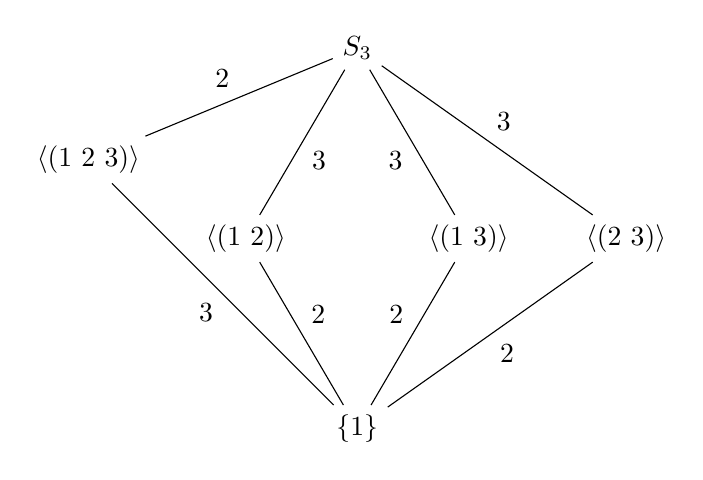
\begin{tikzpicture}[node distance=2cm]
                    \node (S3) {$S_3$};
                    \node (1) [below left of=S3, yshift=-1cm] {$\left\langle (1\ 2)\right\rangle$};
                    \node (2) [below right of=S3, yshift=-1cm] {$\left\langle (1\ 3)\right\rangle$};
                    \node (3) [left of=1, yshift=1cm] {$\left\langle (1\ 2\ 3)\right\rangle$};
                    \node (4) [right of=2] {$\left\langle (2\ 3)\right\rangle$};
                    \node (5) [below right of=1, yshift=-1cm] {$\{1\}$};
                    
                    \draw (S3) -- node[below right] {$3$} (1);
                    \draw (S3) -- node[below left] {$3$} (2);
                    \draw (S3) -- node[above left] {$2$} (3);
                    \draw (S3) -- node[above right] {$3$} (4);
                    \draw (1) -- node[above right] {$2$} (5);
                    \draw (2) -- node[above left] {$2$} (5);
                    \draw (3) -- node[below left] {$3$} (5);
                    \draw (4) -- node[below right] {$2$} (5);
                \end{tikzpicture}
                \caption{Diagrama de Hasse para los subgrupos de $S_3$.}
            \end{figure}

            Como $\langle (1\ 2\ 3) \rangle \lhd S_3$ y ningun otro subgrupo es normal en $S_3$ salvo $A_3$ y $\{1\}$, la única serie de composición de $S_3$ es:
            \begin{equation*}
                S_3 \rhd A_3 \rhd \{1\}
            \end{equation*}
        \item En $D_4$:
            \begin{figure}[H]
                \centering
                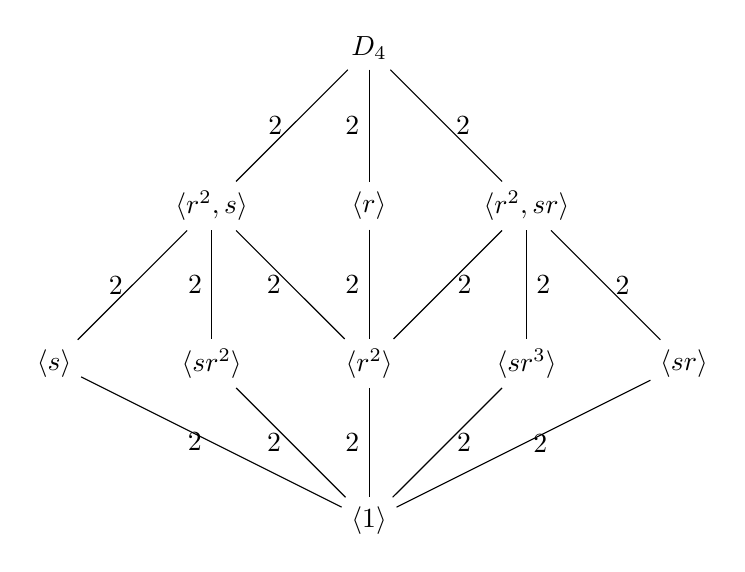
\begin{tikzpicture}[node distance=2cm]
                    \node (D4) {$D_4$};
                    \node[below of=D4] (r) {$\langle r\rangle$};
                    \node[left of=r] (r2s) {$\langle r^2,s\rangle$};
                    \node[right of=r] (r2sr) {$\langle r^2,sr\rangle$};
                    \node[below of=r] (r2) {$\langle r^2\rangle$};
                    \node[left of=r2] (sr2) {$\langle sr^2\rangle$};
                    \node[right of=r2] (sr3) {$\langle sr^3\rangle$};
                    \node[right of=sr3] (sr) {$\langle sr\rangle$};
                    \node[left of=sr2] (s) {$\langle s\rangle$};
                    \node[below of=r2] (1) {$\langle 1\rangle$};

                    \draw (D4) --node[left] {$2$} (r);
                    \draw (D4) --node[left] {$2$} (r2s);
                    \draw (D4) --node[right] {$2$} (r2sr);
                    \draw (r) --node[left] {$2$} (r2);
                    \draw (r2s) --node[left] {$2$} (sr2);
                    \draw (r2s) --node[left] {$2$} (s);
                    \draw (r2s) --node[left] {$2$} (r2);
                    \draw (r2sr) --node[right] {$2$} (sr3);
                    \draw (r2sr) --node[right] {$2$} (sr);
                    \draw (r2sr) --node[right] {$2$} (r2);
                    \draw (r2) --node[left] {$2$} (1);
                    \draw (sr2) --node[left] {$2$} (1);
                    \draw (sr3) --node[right] {$2$} (1);
                    \draw (sr) --node[right] {$2$} (1);
                    \draw (s) --node[left] {$2$} (1);
                \end{tikzpicture}
                \caption{Diagrama de Hasse para los subgrupos de $D_4$.}
            \end{figure}
            Como todos los índices del grafo son 2, todas las relaciones de inclusión mostradas en el grafo en realidad son relaciones de normalidad ($\lhd$), por lo que tenemos 7 series de composición distintas (una por cada forma que tengamos de llegar desde $D_4$ hasta $\{1\}$ en el grafo mediante caminos descendientes):
            \begin{align*}
                D_4 &\rhd \langle r^2, s \rangle \rhd \langle sr^2 \rangle  \rhd \{1\} \\
                D_4 &\rhd \langle r^2, s \rangle \rhd  \langle s \rangle  \rhd \{1\} \\
                D_4 &\rhd \langle r^2, s \rangle \rhd \langle r^2 \rangle  \rhd \{1\} \\
                D_4 &\rhd \langle r^2, sr \rangle  \rhd \langle r^2 \rangle  \rhd \{1\} \\
                D_4 &\rhd \langle r^2, sr \rangle  \rhd \langle sr \rangle  \rhd \{1\} \\
                D_4 &\rhd \langle r^2, sr \rangle  \rhd \langle sr^3 \rangle  \rhd \{1\} \\
                D_4 &\rhd \langle r \rangle \rhd \langle r^2 \rangle  \rhd \{1\}
            \end{align*}
        \item Para $A_4$:

            \begin{figure}[H] % // TODO: Arreglar
                \centering
                \shorthandoff{""}
\begin{tikzcd}
                                                      &                                                     & A_4 \arrow[rrd, "3", no head] \arrow[rdd, "4", no head] \arrow[dd, "4", no head] \arrow[ldd, "4", no head] \arrow[lldd, "4"', no head] &                                                        &                                                                                &                                                         \\
                                                      &                                                     &                                                                                                                                        &                                                        & V \arrow[ldd, "2", no head] \arrow[dd, "2", no head] \arrow[rdd, "2", no head] &                                                         \\
\langle (1\ 2\ 3) \rangle \arrow[rrdd, "3"', no head] & \langle (1\ 2\ 4) \rangle \arrow[rdd, "3", no head] & \langle (1\ 3\ 4) \rangle \arrow[dd, "3", no head]                                                                                     & \langle (2\ 3\ 4) \rangle \arrow[ldd, "3"', no head]   &                                                                                &                                                         \\
                                                      &                                                     &                                                                                                                                        & \langle (1\ 3)(2\ 4) \rangle \arrow[ld, "2"', no head] & \langle (1\ 3)(2\ 4) \rangle \arrow[lld, "2"', no head]                        & \langle (1\ 4)(2\ 3) \rangle \arrow[llld, "2", no head] \\
                                                      &                                                     & \{1\}                                                                                                                                  &                                                        &                                                                                &                                                        
\end{tikzcd}
                \shorthandon{""}
            \end{figure}
            Tenemos como series de composición:
            \begin{align*}
                A_4 &\rhd V \rhd \langle (1\ 2)(3\ 4) \rangle  \rhd \{1\} \\
                A_4 &\rhd V \rhd \langle (1\ 3)(2\ 4) \rangle  \rhd \{1\} \\
                A_4 &\rhd V \rhd \langle (2\ 3)(2\ 3) \rangle  \rhd \{1\} 
            \end{align*}
            Además:
            $\langle (1\ 2\ 3) \rangle > A_4 $ no es una relación normal.
            Por lo que solo tenemos 3 series de composición.
        \item En $D_5 = \langle r,s\mid r^5 = s^2 = 1, sr = r^4 s \rangle $. Tenemos:

            \begin{figure}[H]
                \centering
                \shorthandoff{""}
\begin{tikzcd}
                                             &  & D_5 \arrow[lld, "2", no head] \arrow[dd, "5"', no head] \arrow[rdd, "5"', no head] \arrow[rrdd, "5"', no head] \arrow[rrrdd, "5"', no head] \arrow[rrrrdd, "5", no head] &                                              &                                                 &                                                  &                                                  \\
\langle r \rangle \arrow[rrdd, "5", no head] &  &                                                                                                                                                                          &                                              &                                                 &                                                  &                                                  \\
                                             &  & \langle s \rangle \arrow[d, "2"', no head]                                                                                                                               & \langle sr \rangle \arrow[ld, "2"', no head] & \langle sr^2 \rangle \arrow[lld, "2"', no head] & \langle sr^3 \rangle \arrow[llld, "2"', no head] & \langle sr^4 \rangle \arrow[lllld, "2", no head] \\
                                             &  & \{1\}                                                                                                                                                                    &                                              &                                                 &                                                  &                                                 
\end{tikzcd}
                \shorthandon{""}
            \end{figure}
            Solo tenemos la serie de composición:
            \begin{equation*}
                D_5 \rhd \langle r \rangle  \rhd \{1\}
            \end{equation*}
            Ya que los subgrupos de la derecha no son normales para $D_5$.
        \item En el grupo de los cuaternios:
            \begin{figure}[H]
                \centering
                \begin{tikzpicture}[node distance=2cm]
                    \node (Q2) {$Q_2$};
                    \node (1) [below of=Q2, xshift=-2cm] {$\left\langle i\right\rangle$};
                    \node (2) [below of=Q2] {$\left\langle j\right\rangle$};
                    \node (3) [below of=Q2, xshift=2cm] {$\left\langle k\right\rangle$};
                    \node (4) [below of=2] {$\left\langle -1\right\rangle$};
                    \node (5) [below of=4] {$\{1\}$};

                    \draw (Q2) -- node[above left] {$2$} (1);
                    \draw (Q2) -- node[left] {$2$} (2);
                    \draw (Q2) -- node[above right] {$2$} (3);
                    \draw (1) -- node[below left] {$2$} (4);
                    \draw (2) -- node[left] {$2$} (4);
                    \draw (3) -- node[below right] {$2$} (4);
                    \draw (4) -- node[left] {$2$} (5);
                \end{tikzpicture}
                \caption{Diagrama de Hasse para los subgrupos del grupo de los cuaternios.}
            \end{figure}
            Tenemos 3 series de composición, todos los posibles caminos.
        \item En $S_3\times \mathbb{Z}_2$:
            Por una parte, en $S_3$ teníamos una serie de composición:
            \begin{equation*}
                S_3 \rhd A_3 \rhd \{1\}
            \end{equation*}
            Y en $\mathbb{Z}_2$ la única opción a considerar es $\mathbb{Z}_2 \rhd \{0\}$.
            Podemos considerar ahora las series de composición:
            \begin{align*}
                S_3\times \mathbb{Z}_2 &\rhd S_3 \times \{0\} \rhd A_3\times \{0\} \rhd \{(1,0)\} \\
                S_3\times \mathbb{Z}_2 &\rhd A_3\times \mathbb{Z}_2 \rhd A_3 \times \{0\} \rhd \{(1,0)\} \\
                S_3\times \mathbb{Z}_2 &\rhd A_3\times \mathbb{Z}_2 \rhd \{1\}\times \mathbb{Z}_2 \rhd \{(1,0)\}
            \end{align*}
            Que obtenemos primero variando algunos y luego otras. Esto es posible ya que los subgrupos del producto eran productos de subgrupos, en el Teorema~\ref{teo:grupos_finitos_producto}.

            Como $\mcd(6,2) = 2 \neq 1$, vamos a tener que hay subgrupos que no son producto de uno por producto de otro, por lo que tendremos otra serie de composición:
            \begin{equation*}
                S_3\times \mathbb{Z}_2 \stackrel{2}{\rhd} H_1 \stackrel{2}{\rhd} H_2 \stackrel{3}{\rhd} \{1\}
            \end{equation*}
            Con $H_1\cong S_3$ y $H_2 \cong A_3$.
    \end{itemize}
\end{ejemplo}

\begin{definicion}[Grupo simple]
    Un grupo $G$ se dice simple si no es trivial y no tiene subgrupos normales propios
\end{definicion}

\begin{ejemplo}
    $\mathbb{Z}_3$ es un grupo simple:
    \begin{figure}[H]
        \centering
        \shorthandoff{""}
        \begin{tikzcd}
        \mathbb{Z}_3 \arrow[d, no head] \\
        \{0\}                          
        \end{tikzcd}
        \shorthandon{""}
    \end{figure}
    Un resultado que veremos luego (el Teorema de Abel) nos dirá que los grupos $A_n$ para $n\geq 5$ son grupos simples.
\end{ejemplo}

\begin{prop}
    Un grupo abeliano es simple si y solo si es un grupo cíclico de orden primo.
    \begin{proof}
        Por doble implicación:
        \begin{description}
            \item [$\Longleftarrow)$] Si $G$ es cíclico de orden primo, no va a tener subgrupos propios, por lo que será simple.
            \item [$\Longrightarrow)$] Si $G$ es abeliano, entonces todos sus subgrupos serán normales. Si es simple, no tendrá subgrupos propios (ya que si no serían normales, luego no sería simple). Sea $1\neq x\in G$, sabemos que $\langle x \rangle < G$, de donde $G = \langle x \rangle $, por lo que $G$ es cíclico.

                Si $|G| = nm$, entonces $1\neq \langle x^m \rangle < G$, por lo que $G$ tendría subgrupos propios, luego no sería simple. Por tanto, $|G|$ ha de ser primo.
        \end{description}
    \end{proof}
\end{prop}

\begin{ejemplo}
    Estudiando un poco el caso de grupos cíclicos infinitos, si $G=\mathbb{Z}$, un grupo cíclico finito, $\mathbb{Z}$ no es simple, ya que tiene subgrupos propios (que además son normales, por ser $\mathbb{Z}$ abeliano).
\end{ejemplo}

\begin{prop}
    Si un grupo $G$ tiene una serie de composición, entonces los factores de composición son grupos simples.
    \begin{proof}
        Sea una serie de composición de longitud $r$:
        \begin{equation}\label{eq:prop_1}
            G=G_0 \rhd G_1 \rhd \ldots \rhd G_r = \{1\}
        \end{equation}
        Supongamos que existe un índice $i \in \{1,\ldots,r\}$ de forma que $G_{i-1}/G_i$ no sea un grupo simple. En cuyo caso, existirá un subgrupo normal suyo no trivial $\{1\}\neq H \lhd G_{i-1}/G_i$. Si usamos ahora el 3er teorema de isomorfía para $p:G_{i-1}\to G_{i-1}/G_i$, tenemos que:
        \begin{equation*}
            p_i^\ast(H) \lhd G_{i-1}
        \end{equation*}
        Por lo que hemos encontrado un subgrupo normal que estaría entre $G_i$ y $G_{i-1}$:
        \begin{equation}\label{eq:prop_2}
            G=G_0 \rhd G_1 \rhd \ldots \rhd G_{i-1} \rhd H \rhd G_i \rhd \ldots \rhd G_r = \{1\}
        \end{equation}
        Por lo que~(\ref{eq:prop_2}) es un refinamiento de~(\ref{eq:prop_1}), que era una serie de composición, \underline{contradicción}.
    \end{proof}
\end{prop}

\begin{prop}
    Todo grupo finito tiene una serie de composición.
    \begin{proof}
        Sea $G$ un grupo finito, distinguimos casos en función del orden del grupo:
        \begin{itemize}
            \item Si $|G| = p$ primo, entonces $G$ es simple y tenemos una serie de composición:
                \begin{equation*}
                    G \rhd \{1\}
                \end{equation*}
            \item Si $|G|$ no es primo, por inducción sobre $|G| = n$, suponemos que es cierto para todo grupo $H$ con $|H|<|G|$.

                Como $G$ es finito, tiene un número finito de subgrupos, entre los que podemos encontrar\footnote{Por ser un grupo de orden no primo, no será simple, por lo que tendrá subgrupos normales propios.} $G_1$, un subgrupo normal maximal propio de $G$. Como $|G_1| < |G|$, por hipótesis de inducción tenemos una serie de composición para $G_1$:
                \begin{equation*}
                    G_1 \rhd G_2 \rhd \ldots \rhd G_r = \{1\}
                \end{equation*}
                Además, como $G_1$ era un normal maximal, añadiendo a la serie $G_0 = G$, tenemos:
                \begin{equation*}
                    G = G_0 \rhd G_1 \rhd G_2 \rhd \ldots \rhd G_r = \{1\}
                \end{equation*}
        \end{itemize}
    \end{proof}
\end{prop}

\begin{teo}[de Refinamiento de Schreier]
    Sea $G$ un grupo, dos series normales de $G$ tienen refinamientos isomorfos.
    \begin{proof}
        Consideramos dos series normales de $G$:
        \begin{equation}\label{eq:teo_1}
            G = G_0 \rhd G_1 \rhd \ldots \rhd G_{i-1} \rhd G_i \rhd \ldots\rhd G_r = \{1\} \\
        \end{equation}
        \begin{equation}\label{eq:teo_2}
            G = H_0 \rhd H_1 \rhd \ldots \rhd H_{j-1} \rhd H_i \rhd \ldots \rhd H_s = \{1\}
        \end{equation}
        Para todo $i \in \{1,\ldots,r\}$, tenemos $G_i \lhd G_{i-1} < G$, donde podemos aplicar el primer apartado del Cuarto Teorema de Isomorfía:
        \begin{equation*}
            G_{ij} = G_i(H_j\cap G_{i-1}) \lhd G_i(H_{j-1}\cap G_{i-1}) = G_{ij-1}
        \end{equation*}
        En los extremos:
        \begin{align*}
            G_{i0} &= G_i(H_0\cap G_{i-1}) = G_iG_{i-1} = G_{i-1} \\
            G_{is} &= G_i(H_s\cap G_{i-1}) = G_i \{1\} = G_i
        \end{align*}
        De esta forma, tenemos para todo $i \in \{1,\ldots,r\}$ que:
        \begin{equation*}
            G_{i-1} = G_{i0} \rhd G_{i1} \rhd \ldots \rhd G_{is-1} \rhd G_{is} = G_i
        \end{equation*}
        Que podemos meter en todos los eslabones de la serie~(\ref{eq:teo_1}):
        \begin{multline*}
            G = G_0 = G_{i0} \rhd G_{11} \rhd \ldots \rhd G_{1s} = G_1 = G_{20} \rhd G_2 \rhd \ldots \rhd G_{2s} = G_2 = G_{30} \rhd \ldots  \\
            \rhd G_{r-1s} = G_{r-1} = G_{r0} \rhd \ldots \rhd G_{rs} = G_r =  \{1\}
        \end{multline*}
        Que tiene longitud $r(s+1)-(r-1) = rs + 1$.\\

        \noindent
        Para la serie~(\ref{eq:teo_2}), para todo $j\in \{1,\ldots,s\}$ y para $i \in \{0,\ldots, r\}$, por el Cuarto Teorema de Isomorfía tenemos:
        \begin{equation*}
            H_{ij} = H_j(G_i\cap H_j-1) \lhd H_j(G_{i-1}\cap H_{j-1}) = H_{i-1j}
        \end{equation*}
        En los extremos:
        \begin{align*}
            H_{0j} &= H_{j-1} \\
            H_{rj} &= H_j
        \end{align*}
        Y podemos obtener una serie al igual que antes:
        \begin{equation*}
            H_{j-1} = H_{0j} \rhd H_{1j} \rhd \ldots \rhd H_{s-1j} \rhd H_{sj} = H_j
        \end{equation*}
        Obteniendo:
        \begin{equation*}
            G=H_0=H_{01} \rhd \ldots \rhd H_{rs} = H_s = \{1\}
        \end{equation*}
        Que también tiene longitud $rs +1$.\\

        \noindent
        Ahora, por la segunda parte del Cuarto Teorema de Isomorfía, tenemos que:
        \begin{equation*}
            \dfrac{G_{ij-1}}{G_{ij}} = \dfrac{G_i(H_j\cap G_{i-1})}{G_i(H_j\cap G_{i-1})} \cong \dfrac{H_j(G_{i-1}\cap H_{j-1})}{H_j(G_i \cap H_{j-1})} = \dfrac{H_{i-1j}}{H_{ij}}
        \end{equation*}
        Por lo que los dos refinamientos encontrados son isomorfos.
    \end{proof}
\end{teo}

\begin{ejemplo}
    Se pide calcular:
    \begin{align*}
        G &= G_0 \rhd G_1 \rhd G_2 \rhd G_3 = \{1\} \\
        G &= H_0 \rhd H_1 \rhd H_2 = \{1\}
    \end{align*}
\end{ejemplo}

\begin{teo}[Jordan-Holder]
    Si un grupo $G$ admite una serie de composición, cualquier serie normal puede refinarse a una serie de composición.\\

    \noindent
    Además, dos series de composición de un grupo son isomorfas.
    \begin{proof}
        Tomamos una serie de composición de $G$:
        \begin{equation*}
            G= G_0 \rhd G_1 \rhd \ldots \rhd G_r = \{1\}
        \end{equation*}
        Y también una serie normal de $G$:
        \begin{equation*}
            G=H_0 \rhd H_1 \rhd \ldots \rhd H_s = \{1\}
        \end{equation*}
        Por el Teorema de Schreier (la serie de composición es normal), existe un refinamiento de ambos isomorfo. Sin embargo, como la primera serie es de composición, su refinamiento coincide con ella misma. Para la segunda serie, obtendremos un refinamiento isomorfo a la primera:
        \begin{equation*}
            G = \overline{G_0} \rhd \overline{G_1} \rhd \ldots \rhd \overline{G_r} = \{1\}
        \end{equation*}
    \end{proof}
\end{teo}
